% IEEE layout preview. Use the target venue's template for submission.
\documentclass{IEEEtran}
\usepackage{graphicx}
\usepackage{url}

\title{Student Burnout, Study Conditions, and Generative Artificial Intelligence Use: An Exploratory Prediction Study}
\author{Ali Omar and Abdallah Mestrah%
\thanks{Ali Omar and Abdallah Mestrah are with Lebanese University.}}

\begin{document}
\maketitle

\begin{abstract}
This study examined whether survey questions on generative artificial intelligence (GenAI) use and dependence improved estimates of current student burnout beyond study conditions.
The analysis included 97 cross-sectional survey responses, 87 from students who reported attending universities in Lebanon.
Burnout was measured on a 1-to-5 scale using the 12-item Burnout Assessment Tool for Students.
Both prediction tasks were evaluated using repeated nested cross-validation.
In matched comparisons using the same model type and test students, adding three GenAI questions to five study-condition questions reduced mean absolute error from 0.6183 to 0.5883 points.
Adding all GenAI questions to a broader set of background and study-condition questions reduced error from 0.6145 to 0.5933 points.
A separate comparison evaluated two approaches to identifying students with measured burnout scores of at least 4.
At the selected warning thresholds, the workload-only model detected an average of 16.0 of the 17 high-symptom cases, and the eight-question model detected 14.8.
Both averaged 28 false warnings among the 80 students below the cutoff. The conditional 95\% intervals for paired performance differences included zero.
The eight-question model achieved 76.0\% balanced accuracy, exceeding all 199 shuffled-label results (permutation \(p=0.005\)).
Independent validation is needed to assess whether the findings generalize to other student cohorts.
\end{abstract}


\begin{IEEEkeywords}
Academic burnout, generative artificial intelligence, logistic regression, random forests, university students.
\end{IEEEkeywords}

\section{Introduction}
\label{sec:introduction}

\subsection{Context}

Academic burnout in university students includes exhaustion, detachment from studies, and difficulties with thinking and regulating emotions~\cite{carmonahalty2024bats}. In a survey of Brazilian university students, taking many courses and managing exams and assignments were among the academic demands associated with burnout~\cite{camara2024stressors}. Perceived workload therefore provides a baseline for assessing the value of additional survey responses.

Students use generative artificial intelligence (GenAI) for learning support and to carry out parts of academic tasks. In a survey of Thai undergraduates, academic stress and AI dependence were positively associated with burnout in the same regression model. Evidence of an association was weaker for AI-supported learning~\cite{plensamai2026burnout}. The main goal of this study was to predict current burnout scores and determine whether students' answers about GenAI use, including AI dependence, improve prediction beyond study conditions alone.

\subsection{Prediction Tasks and Evaluation Challenges}

The analysis used a cross-sectional survey of 97 university students, 87 of whom reported enrollment in Lebanon. Symptoms reported at the time of the survey were measured on a scale of 1 to 5 using 12 items from the student version of the Burnout Assessment Tool (BAT-S).

The study had two objectives.

\begin{enumerate}
\item Predict the numerical burnout score and measure the change in prediction error when three GenAI questions are added to five questions about study conditions. The added questions cover GenAI use frequency, dependence on AI to complete academic work, and reliance on AI in place of independent thinking.
\item Identify students with a measured burnout score of at least 4, the study's High group (17 students). Compare a logistic regression model that uses workload alone with a random forest that uses the five study-condition and three GenAI questions. The comparison counts High students detected and warnings issued to students with measured scores below 4.
\end{enumerate}

Prior studies illustrate how the choice of outcome and evaluation sample shapes a prediction study. She et al. defined cutoffs for burnout specific to foreign-language learning and evaluated their models on students from a separate school~\cite{she2026languageburnout}. In a preprint on a combined burnout and depression outcome, Dehghan and Ashrafi showed how overlap between a predictor and part of the outcome can dominate model explanations~\cite{dehghan2026overlap}. In the present study, the predictor sets excluded all BAT-S responses and derived scores. Performance was evaluated on students held out from model fitting within the survey sample.

\subsection{Study Contributions and Main Findings}

Adding the three GenAI questions as a set reduced mean absolute error from 0.6183 to 0.5883 points on the 1-to-5 scale. This comparison used ridge regression and identical evaluation splits for both input sets. Even with the added questions, the model averaged 0.9329 points of error in the High group and tended to underestimate scores there.

At the selected warning thresholds, workload-only logistic regression detected an average of 16.0 of the 17 High cases (94.1\%). The eight-input random forest detected 14.8 cases (87.1\%). Both models averaged 28 false warnings among the 80 students below the cutoff. Warning precision, the percentage of warnings that identified High cases, was 36.4\% for workload-only logistic regression and 34.7\% for the random forest. These figures are averages from five cross-validation repetitions on the same 97 students.

Across warning thresholds, the random forest achieved higher average precision than workload-only logistic regression (0.527 versus 0.423). With the original labels, the random forest achieved 76.0\% balanced accuracy, the mean of the correct classification rates for the two groups. This value exceeded the balanced accuracy of all 199 runs of the selected forest procedure with shuffled labels (permutation \(p = 0.005\)).

In an earlier comparison, the 23-input support vector classifier averaged 19.4 false warnings and detected 13.0 of the 17 High cases. The classifier generated fewer false warnings than the random forest and detected fewer High cases.

\subsection{Paper Structure}

Related Work reviews student burnout measurement, GenAI use, and model interpretation. Study Design and Evaluation describes the survey, outcomes, models, and validation procedure. Results and Discussion presents the model comparisons and their limitations. The conclusion summarizes what the survey results support.

\section{Related Work}
\label{sec:related-work}

\subsection{Measuring Student Burnout}

Student burnout studies differ in both measurement instruments and score cutoffs. Carmona-Halty et al. found support for four BAT-S dimensions in 461 Chilean undergraduates~\cite{carmonahalty2024bats}. Kiss and Pik\'{o} used the Maslach Burnout Inventory--Student Survey with Hungarian medical students and applied separate cutoffs for exhaustion, cynicism, and academic efficacy~\cite{kiss2025burnout}. In the present study, regression estimates the 12-item BAT-S score. The classification task uses a cutoff of 4 on the same score to define the High group.

\subsection{Study Conditions and GenAI Use}

C\^{a}mara and Carlotto found that taking many courses and managing exams and assignments were among the stressors associated with burnout in Brazilian university students~\cite{camara2024stressors}. The present survey measures perceived workload with one question asking how heavy and overwhelming students find their academic workload. This item is the only input to the logistic regression baseline for the warning task.

Measures of GenAI use can describe frequency, purpose, or dependence. Plensamai found a positive association between AI dependence and burnout after adjusting for academic stress and AI-supported learning~\cite{plensamai2026burnout}. In a survey of Chinese university students, Wang et al. found positive correlations between academic stress, AI dependence, and burnout scores~\cite{wang2026offloading}. Both surveys measured these variables at one point in time. The present score prediction experiments compare prediction errors for held-out students with and without GenAI items, using the same model family within each comparison.

\subsection{Comparing Burnout Prediction Models}

Some burnout classifiers use symptom scores as predictors. Rahmadani and Sriani used burnout dimension scores as inputs to a decision tree that classified Indonesian university students into three burnout levels~\cite{rahmadani2026burnout}. In the present study, BAT-S responses define the outcomes, and the prediction models use answers from the other parts of the survey.

Saklani et al. used a 23-item BAT-S mean to define three groups in an analysis of 113 Indian engineering students~\cite{saklani2026burnout}. With the full set of predictors, their logistic regression and random forest models performed better than in the corresponding runs with shuffled labels. The uncertainty intervals for the gains from adding interaction terms included zero. The present study evaluates the selected random forest against runs with shuffled labels to assess performance relative to chance. The comparison with workload-only logistic regression examines High detections and false warnings at the selected thresholds.

\subsection{Interpreting Model Outputs}

She et al. used Shapley additive explanations (SHAP) to interpret their model. Foreign-language enjoyment and academic stress contributed most to its predictions~\cite{she2026languageburnout}.

Predictor rankings can depend on how the outcome is defined. In a preprint, Dehghan and Ashrafi found that trait anxiety fell from first to sixth in a model with a combined burnout and depression outcome after they removed the variance it shared with the depression subscale~\cite{dehghan2026overlap}. Our study compares performance across sets of survey questions and examines prediction errors by symptom level.

\section{Study Design and Evaluation}
\label{sec:study-design-and-evaluation}

Fig.~\ref{fig:study-design} shows the main comparisons for the two prediction tasks.

\begin{figure}[t]
\centering
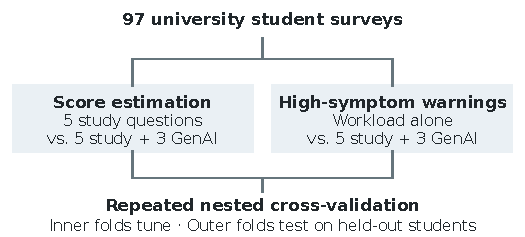
\includegraphics[width=\columnwidth]{figures/study-design.pdf}
\caption{Input sets for score estimation and high-symptom warnings. Numbers in parentheses give input counts.}
\label{fig:study-design}
\end{figure}

\subsection{Participants and Questionnaire}


We used convenience sampling to recruit Lebanese undergraduate and graduate students from multiple universities for an online cross-sectional survey. The survey link circulated primarily through WhatsApp among student contacts and their peers. We assessed eligibility using recruitment information and self-reported answers.

We analyzed all 97 survey submissions received from 4 to 18 October 2026. Of the respondents, 87 reported attending a university in Lebanon. Based on recruitment information, we identified the other 10 as Lebanese students studying abroad. After data collection, we revised the original location-based eligibility rule to include them.

The opening pages of the Google Forms survey explained the study and stated that participation was voluntary. Respondents indicated consent by choosing to continue. The form did not ask for names, contact information, or other direct identifiers. The study was not submitted for formal ethics review.

The questionnaire contained 20 questions on student background, study conditions, GenAI use, and intention to continue studying. It then presented the 23 core items of the English student version of the Burnout Assessment Tool (BAT-S)~\cite{schaufeli2020bat,batsenglishquestionnaire}. Short explanations clarified the word \emph{cynical} in BAT-S item Q33 and \emph{procrastinate} in the separate study-conditions item Q18.

\subsection{Outcomes and Data Preparation}

Responses to every BAT-S item used a scale from 1 (never) to 5 (always), with higher values indicating more frequent symptoms. For both scores, the calculation first averaged the items within each of the four dimensions. The four dimension means then contributed equally to the overall score.

The primary score used the 12 items marked as the short form in the English questionnaire. The secondary score used all 23 core items. Table~\ref{tab:bats-items} lists the survey question numbers for both scores. Each calculation required responses to all of its items, and both scores were complete for all 97 students.

\begin{table}[t]
\caption{Survey Items Used to Calculate the BAT-S Scores}
\label{tab:bats-items}
\centering
\footnotesize
\begin{tabular}{@{}lll@{}}
\hline
Dimension & Primary items & Core items \\
\hline
Exhaustion & Q21, Q23, Q24 & Q21--Q28 \\
Mental distance & Q29, Q31, Q33 & Q29--Q33 \\
Cognitive impairment & Q34, Q37, Q38 & Q34--Q38 \\
Emotional impairment & Q39, Q40, Q43 & Q39--Q43 \\
\hline
\end{tabular}
\end{table}

The warning task used the measured primary score to assign each student to one of two groups. A score of 4 or above defined the High group (17 students). Scores below 4 defined the Below-high group (80 students). Both groups describe symptom levels at the time of the survey.

Data preparation included checking the prepared data against the original export and recalculating the scores. One imported internet rating was corrected from the original answer, and one emotional-impairment mean was recalculated from its component items. When data were loaded for model fitting, three missing indicators of AI use for summarization were reconstructed from the original selections. The recoding completed the model inputs and left the prepared data file unchanged.

IBM SPSS Statistics 23 was used to summarize responses and scores and to calculate Cronbach's alpha for each dimension and for the 12-item and 23-item sets. Two-sided Spearman correlations examined 11 separate associations with the primary score without adjustment for multiple testing. A Pearson correlation was also calculated between AI dependence and the primary score.

\subsection{Input Sets and Score Prediction}

To test whether GenAI questions improved score prediction, we compared input sets using the same model family and evaluation splits within each comparison. Small A used five study-condition questions on perceived workload, sleep duration category, independent study-hours category, financial strain, and university support. Small B added three questions on GenAI use frequency, self-reported dependence on AI to complete academic work, and reliance on AI in place of independent thinking, for eight inputs.

Broad C used 13 inputs on background and study conditions (Q1--Q7 and Q14--Q19). It added eight questions to Small A, covering enrollment location, academic level, major, GPA range, electricity outages, internet quality, academic stress, and avoidance or procrastination.

Broad D added all six GenAI questions (Q8--Q13) to Broad C, covering frequency, use cases, dependence, reliance in place of independent thinking, verification of AI outputs, and concerns about being flagged for AI use. Q9 supplied separate yes-or-no inputs for concept explanations, writing, coding, summaries, and direct solutions, so 19 questions yielded 23 inputs before categorical encoding. All input sets excluded BAT-S responses and scores, submission timestamps, and the item on intention to continue studying.

The Small A and Small B comparison used linear regression, ridge regression, and a shallow random forest. The Broad C and Broad D comparison used ridge regression. The reference predictions were the mean and median measured scores in the training data.

Designated categorical inputs were encoded as separate indicators, with the first response category as the reference. For ridge regression, the encoded inputs were standardized using training data. The ridge penalty ranged from 0.01 to 1000 in tenfold steps. The regression forest used 200 trees, with candidate maximum depths of 2 and 3 and minimum leaf sizes of 5 and 10.

Score prediction used five repetitions of shuffled five-fold cross-validation. Each outer test fold held out one group of students for evaluation. Four inner folds within the remaining training data were used to select model settings by mean absolute error (MAE), the average absolute difference between predicted and measured scores. Predictions were clipped to the 1-to-5 scale during tuning and evaluation. MAE was calculated for the full sample and for students with measured scores of 4 or above.

Follow-up experiments gave more weight to errors for high scores. One comparison used a fixed equal-weight average of predictions from weighted ridge regression on Small B and support vector regression on Broad D.

\subsection{High-Symptom Warning Models}

The selected random forest classifier used Small B to predict the High label directly. The classifier used 100 trees, with candidate maximum depths of 2 and 3, minimum leaf sizes of 5 and 10, and relative training weights for the High group of 1, 2, and 4. The weights were rescaled within each fit to have a mean of 1.

The warning threshold determined when the classifier output triggered a warning. Candidate thresholds ranged from 0 to 1 in increments of 0.05. The separate cutoff of 4 applied to the measured BAT-S score and determined the student's group.

The augmentation procedure tested three quantities of synthetic profiles. It added zero, half as many, or as many profiles as there were real High students in the current training split. Fractional target counts were rounded up. Each synthetic profile was based on two High students from that split.

The distance between two students was the average of eight values. These were the six absolute differences in ordered responses, each divided by four, and two indicators of category mismatch. Eligible pairs had a distance of at most 0.35, and each ordered response differed by at most two points. The first student was selected at random from those with an eligible neighbor. The second was selected at random from up to three of the closest eligible neighbors.

The six ordered responses were interpolated using one shared fraction drawn uniformly from 0.2 to 0.8. Each resulting value was rounded probabilistically to a valid response value. The new profile inherited the first student's sleep and study-hours categories and was assigned a High label. To be accepted, a profile had to fall within 0.25 of the first student. Duplicates of real training profiles or previously accepted synthetic profiles in that split were rejected.

The comparison on real students included an eight-input forest tuned without augmentation. A logistic regression baseline using standardized perceived workload alone was added after the earlier model comparisons. It used \(L_2\) regularization with \(C=1\). The class weights and warning thresholds were selected from the same candidate values as for the forest.

Two fixed reference rules warned everyone or nobody. For the random reference, expected detections and false warnings were calculated for random selection of the same number of students as the forest warned in each outer test fold.

Earlier exploratory comparisons included support vector classifiers with a radial basis function kernel, using Small B or Broad D. These classifiers used real training data and tuned their settings and warning thresholds in the inner folds.

A separate historical fit used all 97 students. Its forest settings were depth 3, a minimum leaf size of 10, a relative High weight of 2, a warning threshold of 0.35, and zero synthetic training rows. The simulation applied this fitted model to 970 interpolated profiles. The profile labels were inherited from the students in the training data. The estimates for real students were obtained from the outer test folds described below.

\subsection{Warning Evaluation and Performance Measures}

The warning evaluation used five repetitions of stratified five-fold cross-validation to keep the proportion of High students similar across outer folds. For each outer test fold, four stratified inner folds within the training data were used to select model settings, class weight, augmentation ratio, and warning threshold where applicable.

Selection used the pooled inner-fold \(F_2\) score, which gives greater weight to recall than precision. Ties favored higher precision, higher recall, a higher warning threshold, and then a smaller augmentation ratio where applicable.

For the forest, the sleep and study-hours categories were encoded and the resulting columns were standardized using the corresponding training data. Synthetic profiles for each fit were generated from the same training split. Only held-out real students contributed predictions to the outer evaluation. The reproduced ridge and warning evaluations used scikit-learn version 1.9.1. The other model comparisons are reported from their analysis records.

The held-out predictions were pooled within each repetition, so each student contributed once per repetition. Recall is the share of High students detected, and precision is the share of warnings issued to High students. Balanced accuracy averages the correct classification rates of the two groups. Average precision and the area under the receiver operating characteristic curve summarized ranking across thresholds. Each measure was averaged across the five repetitions.

The chance comparison shuffled the student labels 199 times while preserving the overall class counts. Each shuffle assigned one label per student across all repetitions. For each shuffle, the stratified splits were rebuilt and the selected forest procedure was repeated, including the inner selection and training-only generation of synthetic profiles. The comparison used mean balanced accuracy, as specified in the validation plan. The one-sided permutation \(p\)-value was \((b+1)/200\), where \(b\) counts shuffled runs that reached or exceeded the observed value~\cite{phipson2010permutation}.

Uncertainty was estimated from 2,000 bootstrap samples. Students were resampled with replacement within each outcome group. Each sampled student carried all five held-out predictions, and the models were compared using the same resamples. The 95\% percentile intervals describe variation conditional on the observed class counts and fitted predictions.

\section{Results and Discussion}
\label{sec:results-and-discussion}

\subsection{Burnout Scores and Survey Associations}

The mean primary BAT-S score was 3.125 (SD 0.795), and the mean secondary score was 3.150 (SD 0.765). Seventeen of the 97 students (17.5\%) met the High criterion of a primary score of at least 4. Cronbach's alpha was 0.900 for the 12 items in the primary score and 0.944 for the 23 core items. Alpha measures how consistently the items in each set vary together.

Among the 11 questions tested, avoidance or procrastination had the largest Spearman correlation with the primary burnout score (\(\rho=0.445\)). Perceived workload and academic stress had correlations of 0.388 and 0.367, respectively. Of the three GenAI questions in the eight-input set, AI dependence had the largest correlation (0.377), followed by reliance on AI in place of independent thinking (0.331) and frequency of use (0.220). These exploratory estimates describe the association between each question and the burnout score, without adjustment for other questions or for multiple testing.

\subsection{Numerical Score Prediction}

The ridge regression comparison evaluated the five- and eight-input sets on the same held-out students. Adding the three GenAI questions reduced mean absolute error (MAE) for the primary score by 0.0300 points, from 0.6183 to 0.5883. For the secondary score, MAE decreased from 0.6001 to 0.5528 points. With the same eight inputs, XGBoost produced higher errors than ridge for both the primary score (0.6155 points) and the secondary score (0.5749 points).

In the matched ridge comparison of the 13- and 23-input sets, adding the GenAI questions reduced MAE from 0.6145 to 0.5933 points for the primary score and from 0.5874 to 0.5578 points for the secondary score. MAE decreased in all five repetitions for both scores. The training-mean and training-median benchmarks had primary-score MAEs of 0.6291 and 0.6262 points, respectively.

Table~\ref{tab:score-prediction-results} compares the primary-score errors for the full sample and the High group. Ordinary ridge with eight inputs tended to underestimate scores in the High group. With the same inputs, weighted ridge reduced High-group MAE from 0.9329 to 0.6649 points and increased overall MAE from 0.5883 to 0.6282 points.

The fixed blend gave equal weight to ridge and support vector regression (SVR). It achieved lower MAE than either component for the full sample and for the High group. Its overall MAE was higher than that of ordinary ridge with eight inputs. Selecting the blend weights in the inner folds increased both errors relative to the fixed blend.

\begin{table}[t]
\caption{Recorded Mean Absolute Error for the Primary Burnout Score}
\label{tab:score-prediction-results}
\centering
\footnotesize
\begin{tabular}{@{}lrr@{}}
\hline
Score procedure & Overall (points) & High (points) \\
\hline
Ordinary ridge, 5 inputs & 0.6183 & 1.0842 \\
Ordinary ridge, 8 inputs & 0.5883 & 0.9329 \\
Ordinary ridge, 13 inputs & 0.6145 & 1.0237 \\
Ordinary ridge, 23 inputs & 0.5933 & 0.9281 \\
Weighted ridge, 8 inputs & 0.6282 & 0.6649 \\
High-priority SVR, 23 inputs & 0.6282 & 0.6705 \\
Fixed ridge/SVR blend & 0.6160 & 0.6422 \\
Inner-selected blend & 0.6343 & 0.6664 \\
\hline
\end{tabular}
\end{table}

\subsection{High-Symptom Warning Performance}

Across five cross-validation repetitions, workload-only logistic regression detected an average of 16.0 of the 17 High students (94.1\% recall), and the eight-question forest detected 14.8 (87.1\% recall). Both averaged 28 false warnings among the 80 Below-high students (Fig.~\ref{fig:warning-counts}). Precision was 36.4\% for workload alone and 34.7\% for the forest.

\begin{figure}[t]
\centering
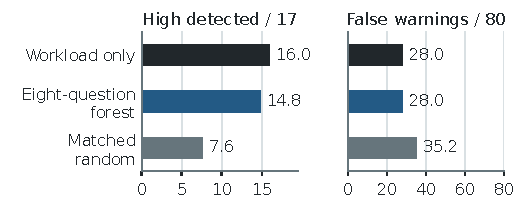
\includegraphics[width=\columnwidth]{figures/warning-counts.pdf}
\caption{Mean detections and false warnings per repetition on held-out students. The random reference shows expected counts when matched to the forest's number of warnings in each test fold.}
\label{fig:warning-counts}
\end{figure}

At the selected thresholds, workload-only logistic regression achieved higher balanced accuracy (79.6\% versus 76.0\%) and a higher \(F_2\) score (0.714 versus 0.668) than the selected forest. Across warning thresholds, the forest achieved higher average precision (0.527 versus 0.423), and workload-only logistic regression achieved a higher area under the receiver operating characteristic (ROC) curve (0.824 versus 0.809).

With training augmentation available during tuning, the forest detected an average of 0.4 more High students and issued 1.6 fewer false warnings than the forest tuned without augmentation.

The permutation test evaluated the selected forest against chance within the study sample (Fig.~\ref{fig:permutation-accuracy}). With the original labels, the forest achieved 76.0\% balanced accuracy. Across the 199 shuffled-label evaluations, mean balanced accuracy was 49.6\% and the maximum was 63.6\%. All shuffled-label results fell below the observed value, yielding a corrected one-sided permutation \(p\)-value of 0.005.

\begin{figure}[t]
\centering
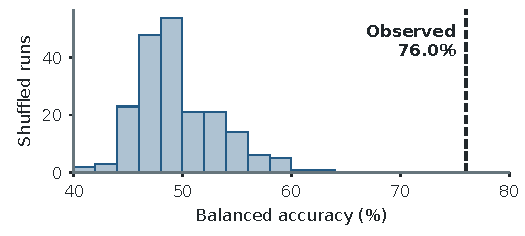
\includegraphics[width=\columnwidth]{figures/permutation-accuracy.pdf}
\caption{Balanced accuracy of the eight-question procedure with the observed labels (dashed line) and across 199 shuffled-label evaluations. Each value averages five cross-validation repetitions.}
\label{fig:permutation-accuracy}
\end{figure}

Table~\ref{tab:warning-intervals} gives conditional intervals for the forest and the paired differences between the forest and workload-only logistic regression. The interval calculation resampled students with the fitted predictions held fixed. All three paired intervals included zero. Across the five cross-validation repetitions, the forest's recall ranged from 82.4\% to 94.1\%, and its false-warning count ranged from 24 to 30.

\begin{table}[t]
\caption{Conditional 95\% Intervals for Warning Performance}
\label{tab:warning-intervals}
\centering
\footnotesize
\begin{tabular}{@{}lrr@{}}
\hline
Metric & \shortstack[b]{Forest\\(\%)} & \shortstack[b]{Forest minus workload\\(percentage points)} \\
\hline
Recall & 70.6 to 100.0 & \(-20.0\) to \(2.4\) \\
Precision & 27.9 to 42.7 & \(-7.3\) to \(3.1\) \\
Balanced accuracy & 66.4 to 83.8 & \(-11.1\) to \(2.3\) \\
\hline
\end{tabular}
\end{table}

\subsection{Earlier Warning Comparisons and Synthetic Check}

Earlier experiment records show the trade-off between detecting High students and issuing false warnings. Under \(F_2\) tuning, the 23-input support vector classifier averaged 13.0 High detections and 19.4 false warnings. The forest fitted with inputs selected by Boruta~\cite{kursa2010boruta} averaged 12.4 High detections and 22.2 false warnings. Both procedures detected fewer High students than the selected forest.

In an earlier comparison using the same eight inputs, TabPFN-2~\cite{hollmann2025tabpfn} had higher average precision (0.616) than the selected forest. The TabPFN-2 rule selected using \(F_2\) averaged 13.8 High detections and 24.2 false warnings. The rule tuned to favor recall averaged 15.2 High detections and 44.0 false warnings.

The synthetic check used 970 profiles generated from survey responses already used to fit the model. The model fitted on all 97 students flagged 159 of the 170 profiles assigned a High label (93.5\%). This rate measures agreement with the High labels inherited from the source responses.

\subsection{Discussion}

The measured reduction in ridge regression error applies to the three GenAI questions together. AI dependence had the strongest individual association with the burnout score among those three questions. Plensamai reported a positive association in the same direction among Thai undergraduates using a different burnout measure~\cite{plensamai2026burnout}. An additional matched comparison that adds AI dependence alone would be needed to estimate its individual contribution to prediction.

At the chosen warning thresholds, workload-only logistic regression detected more High cases at the same average false-warning count as the random forest. The warning comparison varied both the classifier and the inputs, so these results compare the two procedures as a whole.

About two of every three warnings from the selected forest went to students with a burnout score below the study cutoff. Of the 80 Below-high students, 39 received at least one false warning across the five repetitions, and 27 received a false warning in at least three repetitions.

The survey measured GenAI habits, study conditions, and symptoms at one time. The order of events therefore remains unresolved. The convenience sample contained 17 High cases, and several model and input choices followed earlier analyses of the same students. The permutation test applies to the selected forest procedure, and the paired intervals apply to its comparison with workload-only logistic regression. Estimating warning performance in a new cohort requires fixing each procedure in advance and evaluating it on independently recruited students with measured BAT-S outcomes.

\section{Conclusion}
\label{sec:conclusion}

Survey questions about generative artificial intelligence use and dependence modestly improved estimates of current burnout scores in this sample of 97 university students. Adding the three questions to the study-condition inputs reduced mean absolute error from 0.6183 to 0.5883 points on the 1-to-5 scale in the matched comparison. The reduction applies to the questions as a set. Average error remained higher in the High group at 0.9329 points.

For the warning task, workload-only logistic regression detected 16.0 of the 17 High cases on average. The eight-input random forest detected 14.8. Both classifiers averaged 28.0 false warnings among the 80 students whose measured score was below 4. In a separate comparison against chance, the selected forest's balanced accuracy was higher than in any of the 199 evaluations with shuffled labels (permutation \(p=0.005\)).

The warning counts are averages from five cross-validation repetitions on a single convenience sample. An independent evaluation should fix the prediction procedures in advance and test them on a new student cohort with measured BAT-S scores.


\section*{Acknowledgment}
We used OpenAI Codex to draft and revise parts of the Abstract, Introduction, Related Work, Study Design and Evaluation, Results and Discussion, and Conclusion. We also used it to write the script that generates the figures.

\bibliographystyle{IEEEtran}
\bibliography{references}
\end{document}
